\documentclass[conference]{IEEEtran}

\makeatletter
% IEEEtran.cls defines \labelindent for backward compatibility reasons
% Undefine \labelindent to allow the use of package enumitem
\let\labelindent\relax
\makeatother


\usepackage[T1]{fontenc}
\usepackage[para]{footmisc}
\usepackage[pdftex]{graphicx}
\usepackage[utf8]{inputenc}
\usepackage{array}
\usepackage{balance}
\usepackage{booktabs}
\usepackage{cite}
\usepackage{color}
\usepackage{comment}
\usepackage{enumitem}
\usepackage{framed}
\usepackage{listings}
\usepackage{microtype}
\usepackage{subcaption}
\usepackage{url}
\usepackage{floatrow}
% Table float box with bottom caption, box width adjusted to content
\newfloatcommand{capbtabbox}{table}[][\FBwidth]


% SQUEEZE
%\addtolength{\parskip}{-1pt}


\definecolor{lightred}{RGB}{150,0,0}
\definecolor{lightgreen}{RGB}{0,150,0}
\definecolor{lightblue}{RGB}{0,0,150}

\lstdefinelanguage{diff}{
  morecomment=[f][\color{lightblue}]{diff },
  morecomment=[f][\color{lightblue}]{index },
  morecomment=[f][\color{lightblue}]{@@},     % group identifier
  morecomment=[f][\color{lightred}]-,         % deleted lines
  morecomment=[f][\color{lightgreen}]+,       % added lines
  morecomment=[f][\color{lightblue}]{---},    % Diff header lines (must appear after +,-)
  morecomment=[f][\color{lightblue}]{+++},
}
\hyphenation{}

\newcommand{\attn}[1]{{\color{red}#1}}
\newcommand{\desc}[1]{{\emph{\color{blue}#1}}}
\newcommand{\needcite}{\attn{\tiny{[cite]}}}
\newcommand{\todo}[1]{\strut\smash{\colorbox{yellow}{\bf TODO: #1}}}
\setlength\OuterFrameSep{0.5em}
\setlength\FrameSep{0.5em}

\begin{document}
\title{Exploring the Use of Deep Learning\\ for Feature Location}
\author{
    \IEEEauthorblockN{
        Christopher S.\ Corley
    }
    \IEEEauthorblockA{
        The University of Alabama\\
        Tuscaloosa, AL, USA\\
        cscorley@ua.edu
    }
    \and
    \IEEEauthorblockN{
        Kostadin Damevski
    }
    \IEEEauthorblockA{
        Virginia State University\\
        Petersburg, VA, USA\\
        damevski@acm.org
    }
    \and
    \IEEEauthorblockN{
        Nicholas A.\ Kraft
    }
    \IEEEauthorblockA{
        ABB Corporate Research\\
        Raleigh, NC, USA\\
        nicholas.a.kraft@us.abb.com
    }
}


\maketitle

\begin{abstract}

Deep learning models are a class of neural networks. Relative to n-gram models,
deep learning models can capture more complex statistical patterns based on
smaller training corpora. In this paper we explore the use of a particular deep
learning model, document vectors, for feature location.  Document vectors seem
well suited to use with source code, because they both capture the influence of
context on each term in a corpus and map terms into a continuous semantic space
that encodes semantic relationships such as synonymy. We present
preliminary results that show that a feature location technique (FLT) based on
document vectors can outperform an analogous FLT based on latent Dirichlet
allocation and then suggest several directions for future work on the use of
deep learning models to improve developer effectiveness in feature location. 

\end{abstract}

\begin{IEEEkeywords}
deep learning;
neural networks;
document vectors;
feature location
\end{IEEEkeywords}

\section{Introduction}\label{introduction}

% 
%  ii.) What is feature location? Breifly, what is the feature
%  Location Current State of the Art / Practice *mainly bag of words
%  approaches
%
When starting a maintenance task, software developers commonly need to
locate the relevant features in a potentially large and unfamiliar
code base. Due to the difficulty and importance of this task,
researchers have proposed a number of approaches to improve
developers' effectiveness in locating features, largely based upon
applying natural language analysis or text retrieval techniques to source
code~\cite{dit_feature_2013}. Most of the proposed feature location
techniques have treated source code as an unordered set of natural
language terms (i.e., as a bag-of-words), even though recent fundamental
results have shown that source code contains context and flow that is
even more pronounced than natural language
text~\cite{hindle_naturalness_2012}.


%
%  What are the contributions of this paper and this line of work
%
In this paper, we explore the use of deep learning, a particular class
of neural networks that has shown promising results in modeling
natural language~\cite{mikolov_distributed_2013}, for feature
location. In particular, we investigate the efficacy of document
vectors~\cite{le_distributed_2014} (DVs). DVs capture the influence of
the surrounding context, and its order, on each term, which can
improve the ranking of results retrieved for a developer
query~\cite{hill_use_2014}. For example, in the statement {\sf
diagram.redraw()} the word {\em diagram} is relevant to the word {\em
redraw} and this relationship is captured by DVs. Therefore, when
querying for {\em diagram}, program elements where {\em redraw} is
also present are considered more relevant and thus are boosted in the
rankings.

Deep learning models such as DVs also create a novel notion
of semantic similarity between the source code terms. Semantic
similarity is the result of mapping the corpus terms into a continuous
semantic space, where synonyms, antonyms, and other semantic relations
are encoded and easily composed together~\cite{le_distributed_2014}.


%
% The results
%

In our preliminary evaluation, we compare a feature location technique (FLT) based on DVs to an FLT based on latent Dirichlet allocation (LDA) using the benchmark by Dit et al.~\cite{Dit-etal_2013}.
The benchmark comprises 633 features from six versions of four open source Java projects, and our results show that for many of the features, the DV-based FLT outperforms the LDA-based FLT.
Our results also show that less time is needed for model training and inference in the DV-based FLT as compared to the LDA-based FLT.
We also suggest directions for future work on the use
of DVs (or other deep learning models) to improve the effectiveness of feature location engines.





\section{Background}\label{background}

%   i.) Describe all the steps of a Deep Learning FL system
%
%

%how do FL systems work in general?
%
Feature location systems retrieve a ranked list of program elements (e.g.,
methods or classes) for a developer query. In the {\em training} phase, feature
location systems construct a model of the software, at the granularity
of program elements, based on the natural language embedded in identifiers and
comments. In the {\em retrieval} phase, given a natural language query, feature
location systems use the model to retrieve the relevant program elements
with high similarity to the query.

\subsection{Feature Location Workflow}

%how does a deep learning system differ
%
A feature location system based on deep learning, during its training phase,
creates a contextual representation of the natural language terms embedded in
the source code. This contextual representation includes influence from terms
preceding and following each term, relative to their distance from that term.
More intuitively, such models incorporate mutual influence between terms in the
same method, while terms that are closer in distance (e.g. occur the same
statement) influence each other more strongly.


\begin{figure}[tb]
\centering
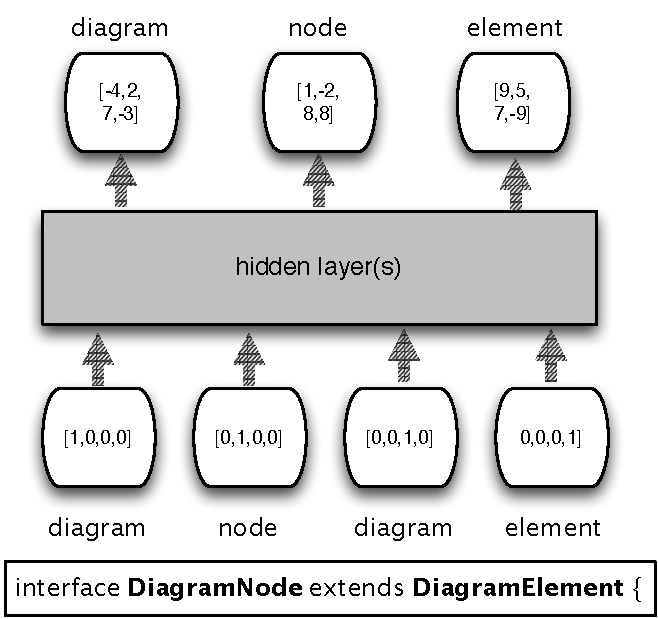
\includegraphics[width=.9\columnwidth]{figures/neuralnet.pdf}
\caption{A deep learning neural network encodes source code identifiers, in the
order they appear in the source code, in its input layer. Using a deep
structure of hidden layers, each term and its context receives a semantic
vector representation. The output layer consists of vector for each term in
the corpus; the vector feature size is arbitrary and does not need to relate to
the number of terms in the corpus.
\vspace*{-2mm}
}
\label{fig:neuralnet}
\end{figure}


%what is deep learning
Deep learning is based on a multi-stage neural network, consisting of several
hidden layers in addition to single input and output layers.  The input layer
consists of an ordered sequences of identifiers extracted from the code. The
multiple hidden layers serve to capture the context for each encountered term,
representing the complex patterns of term contexts occurring in the corpus. The
output layer consists of a vector for each term, which has been shown to carry
semantic meaning. An example of this architecture for a single line of code is
shown in Figure~\ref{fig:neuralnet}. Recent advances in this area have stemmed
from the use of novel neural network architectures, including recurrent neural
networks that connect the hidden layers back to the input layer, among other
strategies. The systems are trained using backpropagation and gradient descent,
techniques common to many neural network based models.

%paragraph2vec
An extension to learning the semantic vector representation of words is the use
of an additional vector that will encode the representation of a larger body of
text, such as a paragraph or an entire document~\cite{le_distributed_2014}.
While comparing word vectors indicates semantic relations between two terms,
comparing two document vectors carries a similar semantic connotation at the
document level. For instance, the approach has been applied for determining the
sentiment (i.e. positive, negative) of reviews on a popular movie recommendation
site.

%preprocessing
A number of preprocessing steps are commonly performed before the training phase
of feature location systems.  
The steps commonly used are~\cite{Marcus-etal_2004,Marcus-Menzies_2010}: % that we use are:
\begin{itemize}
    \item {\it Splitting}: separate tokens into constituent words based on
        common coding style conventions (e.g., the use of camel case or
        underscores) and on the presence of non-letters (e.g., punctuation or
        digits)
    \item {\it Normalizing}: replace each upper case letter with the
        corresponding lower case letter
    \item {\it Filtering}: remove common words such as articles (e.g., `an' or
        `the'), programming language keywords, standard library entity names, or
        short words
\end{itemize}
\newpage

%retrieval
During the retrieval state of feature location, a similarity measure (e.g.
cosine similarity) between the words in the query and words in each program
element is computed. The program elements are ranked based on this similarity
metric and presented to the developer in descending order.

If document vectors are used then a special inference process is needed to infer
a vector representation for the entire query, treated as a document in the
corpus. Following this, the vectors of the query and each program element (i.e.
method or class) can be compared to produce the final ranking.

\subsection{Semantic Similarity}


\begin{table*}[tb]
\centering
\small
\caption{Examples of semantically similar terms and their weight for a deep model trained on
the ArgoUML code base. Only terms with weight > 0.6 are included.}
\label{tab:semsim}
\begin{tabular}{|p{0.30\textwidth}|p{0.60\textwidth}|}
\hline \hline
{\em Term(s)} & {\em Semantically Similar Terms and Weight}\\ \hline \hline
association & (roles 0.75), (role 0.72), (classifier 0.72), (connection, 0.61) \\ \hline
save & (saved 0.69), (pcs 0.64), (exists 0.63), (projects 0.60), (close 0.61), (file 0.60) \\ \hline
file & (filter 0.78), (zip 0.74), (exists 0.74), (persister 0.71), (files 0.69), (directory 0.69) \\ \hline
file + save & (exists 0.77), (saved 0.74), (filter 0.73), (zip 0.72), (unable 0.67), (projects 0.67), (persister 0.67), (files 0.66), (cant 0.66), (scheme 0.65) \\ \hline
explorer + diagrams - creating & (nodes 0.71), (deletion 0.67), (perspectives 0.65), (perspective 0.60), (updated 0.60), (modified 0.60)\\
\hline \hline
\end{tabular}
\end{table*}

The result of the deep learning models described in this paper are vectors
representing each term in the corpus~\cite{mikolov_distributed_2013}. Similar
vectors can also be computed to represent an entire paragraph or
document~\cite{le_distributed_2014}. Semantic similarity is the notion that
these vectors are composable semantically, e.g., the result of the operation
{\em vec(``The Eiffel Tower'') - vec(``Paris'') + vec(``London'')} is closest to
{\em vec(``Big Ben'')}. This capability is established automatically by the
system, without any additional processing or supervised input.

In feature location, as in general information retrieval, the retrieval quality
can only be as good as the quality of the developer query. Problems such as the
dictionary mismatch problem, as well as the propensity of users to issue short
queries, have previously been observed as common difficulties in using feature
location tools in the field~\cite{haiduc_effect_2011, damevski_field_2015}.
Semantic similarity can be a useful capability in mitigating these problems, by
performing query recommendation that allows the user to extend his or her
queries with terms from the same corpus, or automatic query extension.

To illustrate this capability for source code-based corpora, we provide a set of
illustrative examples gathered on the ArgoUML v0.22 in Table~\ref{tab:semsim}.
In many cases semantic similarity provides reasonable results for similar terms,
though exceptions exist largely due to the limited appearance of certain words
in the corpus.  We anticipate that larger corpora, based on larger code bases,
or leveraging related code bases or documents, could improve the results of
semantic similarity even further.




\section{Preliminary Study}\label{study}

%     (compare to LDA and VSM)
%     i. effectiveness on gold sets (F-measure; Mean Average Precision & Precision at Rank 1?)
%	*the deep learning works better as the number of terms grows, so make sure those characteristics come out
%
%     ii. speed
%           (for corpus building; for retrieval)


%
% Notes for Chris and Nick:
% 1) would be nice to also see the number of terms and number of unique terms per each project
% 2) i would definitely show both word2vec and doc2vec features and compare to LDA and VSM
% 3) make sure you mention the exact configuration of preprocessing steps (e.g. no word stemming)
%
\subsection{Subject software systems}

All of our subject software systems come from two publicly-available datasets.
The first is a dataset of six software systems by Dit et
al.~\cite{Dit-etal_2013} and contains method-level goldsets.  This dataset was
automatically extracted from changesets that relate to the queries (issue
reports).

\begin{table}[t]
\renewcommand{\arraystretch}{1.3}
\footnotesize
\centering
\caption{Subject System Sizes and Queries}
\begin{tabular}{lrrr}
    \toprule
    Subject System     & Methods & Queries    \\    %& Goldset Methods
    \midrule                                        %
    ArgoUML v0.22      & 12353    & 91        \\    %& 701
    ArgoUML v0.24      & 13064    & 52        \\    %& 357
    ArgoUML v0.26.2    & 16880    & 209       \\    %& 1560
    Jabref v2.6        & 5357     & 39        \\    %& 280
    jEdit v4.3         & 7305     & 150       \\    %& 748
    muCommander v0.8.5 & 8799     & 92        \\    %& 717
    \midrule                                        %
    Total              & 63758    & 633       \\    %& 4363
    \bottomrule
\end{tabular}
\label{table:subjects}
\end{table}


ArgoUML is a UML diagramming tool\footnote{\url{http://argouml.tigris.org/}}.
jEdit is a text editor\footnote{\url{http://www.jedit.org/}}.
JabRef is a BibTeX bibliography management tool\footnote{\url{http://jabref.sourceforge.net/}}.
muCommander is a cross-platform file manager\footnote{\url{http://www.mucommander.com/}}.

\subsection{Methodology}


\subsection{Setting}

\subsection{Data Collection and Analysis}

\subsection{Results}

\begin{table}
    \centering
\begin{tabular}{llccccc}
\toprule
System & Model &     100 &    200 &    300 &    400 &    500 \\
\midrule
                   &             LDA & 0.0175 & 0.0295 & 0.0271 & 0.0611 & 0.0220 \\
ArgoUML v0.22      & D2V Inference   & 0.0115 & 0.0105 & 0.0096 & 0.0184 & 0.0162 \\
                   & D2V Summation   & 0.0775 & 0.0570 & 0.0625 & 0.0587 & 0.0601 \\
                     \midrule
                   &             LDA & 0.0441 & 0.0373 & 0.0655 & 0.0779 & 0.0344 \\
ArgoUML v0.24      & D2V Inference   & 0.0246 & 0.0152 & 0.0260 & 0.0258 & 0.0380 \\
                   & D2V Summation   & 0.0827 & 0.0906 & 0.0874 & 0.0691 & 0.0942 \\
                     \midrule
                   &             LDA & 0.0493 & 0.0628 & 0.0857 & 0.0703 & 0.0811 \\
ArgoUML v0.26.2    & D2V Inference   & 0.0404 & 0.0218 & 0.0290 & 0.0364 & 0.0403 \\
                   & D2V Summation   & 0.0847 & 0.0890 & 0.0813 & 0.0834 & 0.0805 \\
                     \midrule
                   &             LDA & 0.0055 & 0.0364 & 0.1304 & 0.0781 & 0.0548 \\
JabRef v2.6        & D2V Inference   & 0.0262 & 0.0463 & 0.0318 & 0.0289 & 0.0234 \\
                   & D2V Summation   & 0.0450 & 0.0373 & 0.0455 & 0.0382 & 0.0428 \\
                     \midrule
                   &             LDA & 0.0670 & 0.0432 & 0.0641 & 0.0693 & 0.0607 \\
jEdit v4.3         & D2V Inference   & 0.0341 & 0.0282 & 0.0369 & 0.0354 & 0.0450 \\
                   & D2V Summation   & 0.0872 & 0.0791 & 0.0825 & 0.0814 & 0.0679 \\
                     \midrule
                   &             LDA & 0.0392 & 0.0217 & 0.0198 & 0.0559 & 0.0329 \\
muCommander v0.8.5 & D2V Inference   & 0.0977 & 0.0771 & 0.0800 & 0.0665 & 0.0838 \\
                   & D2V Summation   & 0.0652 & 0.0623 & 0.0703 & 0.0606 & 0.0538 \\

\bottomrule
\end{tabular}
\caption{MRR}
\label{tab:mrr}
\end{table}

\begin{table}
\centering
\begin{tabular}{lcc}
\toprule
                {} & LDA    & Doc2Vec \\
\midrule
ArgoUML v0.22      &  0m 58.207s     &  0m 02.070s     \\
ArgoUML v0.24      &  1m 05.507s     &  0m 02.267s     \\
ArgoUML v0.26.2    &  1m 21.176s     &  0m 02.736s     \\
JabRef v2.6        &  0m 29.504s     &  0m 01.280s     \\
jEdit v4.3         &  0m 36.701s     &  0m 01.519s     \\
muCommander v0.8.5 &  0m 42.897s     &  0m 01.696s     \\
\bottomrule
\end{tabular}
\caption{Model training times for 100 topics}
\end{table}


\begin{table}
\centering
\begin{tabular}{lccc}
\toprule
                {} & LDA    & Vec Inference & Vec Sums \\
\midrule
ArgoUML v0.22      & 0.943362s      &  0.225868s     &  2.118835s         \\
ArgoUML v0.24      & 1.686980s      &  0.259615s     &  1.824923s         \\
ArgoUML v0.26.2    & 0.744468s      &  0.300956s     &  2.715062s         \\
JabRef v2.6        & 0.957000s      &  0.124128s     &  0.720589s         \\
jEdit v4.3         & 0.405700s      &  0.134080s     &  1.017060s         \\
muCommander v0.8.5 & 0.685543s      &  0.165663s     &  1.056108s         \\
\bottomrule
\end{tabular}
\caption{Average time to rank per query for 100 topics}
\end{table}



\subsection{Discussion}


% conclusing remarks:
%   doc2vec faster, could be easier to implement directly into an IDE search
%   tool
%   doc2vec inference needs more exploration for parameter tweaking
%   doc2vec vector summation, although slower, is at an acceptable time


\section{Related Work}\label{related}



%
%  Describe deep learning for natural language
%
Statistical natural language models, such as the n-gram model, have
seen widespread use for a variety of natural language processing tasks
due to their simplicity and effectiveness when trained with a
substantial corpus of text.  Software engineering researchers have
shown n-gram models to be even more effective for source code than for
natural language documents~\cite{hindle_naturalness_2012}. 


Recent research in natural language modeling has introduced deep learning
methods, consisting of specific classes and architectures of neural networks,
that can produce capable statistical models of natural language text able to
capture more complex patterns while being trained using smaller corpora relative
to the n-gram model~\cite{mikolov_distributed_2013,le_distributed_2014}. Using
a set of optimizations strategies such models can be built at reasonable
computational costs.  In this paper we examine the effectiveness and potential
applicability of these deep learning models for the problem of feature location
in software engineering.


%  ii.) What is related work using deep learnign in SE?
%    in S.E. White's paper

White et al.~\cite{white_toward_2015} reported promising results in applying
deep learning models for source code, outperforming models based on similar
n-gram configurations on code completion tasks. This work establishes the use of
deep learning for software engineering problems, sketching out several avenues
for future use of such models, including code completion and the building of
synonym dictionaries, among others. Our work explores these models for the
feature location problem during software maintenance. A notable difference to
the prior experiments conducted by White et al. is that the deep models in this
paper are based solely on terms found in identifiers and comments in the source
code of a single software project, while White et al. considered a larger corpus
consisting of the entire source listing of several combined projects.


%  iii.) Context based approaches to feature location
%	*Emily Hill et al. “One the use of Positional Proximity for IR-Based Feature Location”
%       *Shepherd
%       *SWUM
%       *Naturalness

Previous feature location techniques that incorporated surrounding context in
the model have shown high degrees of effectiveness. Examples include the use of
verb and direct object pairs~\cite{shepherd_using_2007} and statement level
markov random fields~\cite{hill_use_2014}. Deep learning approaches allow the
inclusion of broader context than these previous approaches.

Howard at al.~\cite{howard_automatically_2013} utilized rules based on natural
language text in leading method comments to mine synonym dictionaries from
source code repositories. One of the additional capability of deep language
models is the ability to mine such terms at a greater scale relative to the
their approach.


\section{Conclusions and Future Work}\label{conlusion}

%future work: 
%try in the field (e.g. in Sando)
%maybe try at larger scale 
%incorporate program structure information
%paragraph for each new problem in feature location that this could help (e.g. recommendation)
%Context (compare to n-gram, V-DO stuff)
%

% conclusing remarks:
%   doc2vec faster, could be easier to implement directly into an IDE search
%   tool
%   doc2vec inference needs more exploration for parameter tweaking
%   doc2vec vector summation, although slower, is at an acceptable time


In this work we present a preliminary study of a deep-learning-based
FLT using document vectors (\dv). We find that training the \dv\ 
model has low computational overhead (i.e., is fast), while maintaining
accuracy on par with LDA. We find \dv\ to be a promising solution to implementing
smarter developer search tools in the IDE, a task to which more computationally-intensive models such as LDA are less well-suited.

%Future work includes investigating the approaches performance at differing granularities.
%Additionally, work is needed to investigate effective parameter configurations for the model.
One direction for future work is to explore the effects of parameter tuning on the performance of \dv.
Multiple studies~\cite{Biggers-etal_2014,Panichella-etal_2013a} show that selection of appropriate parameter values is key to the performance of an LDA-based FLT.
Thus, the first question to address is whether the same is true of a \dv-based FLT, and if so, the next question is how to select \dv\ parameters for a particular subject system.
The results of our study show that a \dv-based FLT can provide better accuracy than an LDA-based FLT while requiring fewer computational resources, and more intelligent parameter selection for \dv\ could further improve its accuracy.

Another direction for future work is to use the semantic relations encoded by a \dv\ model for query recommendation or refinement.
We would like to investigate the efficacy of these semantic relations for recommending query terms based on a partial query.
That is, while a developer is entering a query, a recommender could use a \dv\ model of the subject system to recommend additional query terms.
Such an approach would be similar (in function) to the ones implemented in the Sando~\cite{Shepherd:2012} and CONQUER~\cite{CONQUER_2013}.
Similarly, given its relative computational efficiency, using \dv\ as the basis for an IDE-based search tool is a realistic goal.

Further directions for future work include extending the \dv\ model to incorporate program structure information,
an approach which has shown useful when combined with text retrieval models~\cite{Panichella-etal_2013,Saha-etal_2013,Bassett-Kraft_2013},
or extending the \dv\ model to incorporate natural language information such as part-of-speech tags~\cite{Fry-etal_2008} or phrasal representations~\cite{Hill-etal_2011}.


%\section*{Acknowledgments}
%We acknowledge noone.

\bibliographystyle{IEEEtran-nourl}
\bibliography{doc2vec}

\end{document}
